The vague context-dependent nature of gradable adjectives has been promisingly formalized in models within the Rational Speech Act framework -  a suite of game-theoretically oriented recursive models of pragmatic language understanding \parencite[e.g.,][]{goodman2016, lassiter2017adjectival, tessler2017warm}. Introduced by \textcite{frank2012predicting}, the Rational Speech Act framework is well in line with recent insights in the increasingly influential Bayesian cognitive modelling tradition, showing a great deal of flexibility to account for various pragmatic phenomena like scalar implicature, hyperbolic language or generics, among many others \parencite[e.g.,][]{tenenbaum2011grow, problang}. This chapter reviews the Rational Speech Act framework and prior models of gradable adjectives, to finally propose a minimal extension of existing models formalizing the reference-predication trade-off hypothesis, allowing to flexibly incorporate reasoning about context and role of the noun in comparison class inference. 
  
\section{Understanding Rational Speech Act Models}

Language is fascinatingly flexible and efficient; this is largely due to the fact that interlocutors do not have to encode all information explicitly in utterances they produce, but instead rely on each other's ability to infer many aspects of meaning from linguistic and situational context. In particular, pragmatic models of communication posit that given these contextual constrains, speakers and listeners can efficiently \emph{reason about each other's intended meaning} under one important assumption: speakers are approximatly \emph{rational} with respect to their intended goal \parencite{frank2012predicting}. The Rational Speech Act approach (henceforth: RSA) views communication as recursive reasoning between speaker and listener: in interpretation-oriented models, a pragmatic listener $L_1$ infers a state of the world intended to be conveyed by a speaker via the utterance he received, by using \emph{Bayesian inference} to reason about likely world states given the observed utterance, as produces by a pragmatic speaker $S_1$, knowing that $S_1$ chooses the utterance according to its most likely semantic interpretation by a literal listener $L_0$.  

The idea of language as a form of rational action produced by \emph{cooperative} interlocutors was formulated by \textcite{grice1975logic}. At the core of his proposal are four conversational maxims that speakers are thought to stick to when producing utterances in order to convey particular messages: the \emph{maxim of relation} (contributions made to the conversation are relevant), \emph{quantity} (the contributions are as informative as required, but not more so), \emph{quality} (speaker believes their contributions to be true) and \emph{manner} (the way the contributions are expressed is perspicuous). 

Grice’s ideas became particularly influential when precise information-theoretic formalisations of such vague concepts like \emph{informativeness, cooperation} and \emph{relevance} were proposed, and, informed by insights from game-theory, gave rise to RSA \parencite{frank2012predicting}.
In particular, RSA proposes that coordination of intended meaning between interlocutors can be captured via iterative application of probabilistic mechanisms, and context-dependence of meaning can be captured as listener uncertainty about the message encoded in utterances by the speaker (i.e., the state of affairs in the world she wishes to communicate) - in Bayesian cognitive modelling spirit as \emph{subjective beliefs} of the listener - that is, as a \emph{probability distribution} over possible states of the world \parencite{tenenbaum2011grow}. The listener agent $L_1$ can then update her beliefs via Bayes' rule, upon learning a proposition - namely upon hearing an utterance $u$ produced by an informative speaker $S_1$ \parencite{frank2012predicting}.

These mechanisms of RSA are best illustrated by a simple example from a reference game, as described by \textcite{frank2012predicting}:
Consider a simple world consisting of a blue square, a blue circle and a green square (Fig. \ref{rsa-scene}).
\begin{figure*}[t]
	\begin{center}
		
\includegraphics[width=0.5\linewidth]{rsa_scene.png}
	\end{center}
	\vspace{-0.3cm}
	\caption{A simple reference resolution example scenario: the context $C$ consists of three possible referents \parencite{frank2012predicting}}
	\label{rsa-scene}
\end{figure*}
In such a reference game scenario, a speaker wants to communicate to a listener a particular referent $s$ in context $C$, in this toy scenario - one of the items among $C = \{blue-square, blue-circle, green-square\}$  (e.g., the blue square). To do so, she has a finite set of utterances $U = \{blue, green, square, circle\}$.  \footnote{The finite set of alternative utterances is a crucial assumption made in RSA. It is a highly relevant question for future research how human interlocutors actually determine the set of relevant alternatives.} A listener then tries to recover the intended referent (i.e., the blue square) upon receiving an utterance (e.g., "blue"). 
As briefly mentioned above, standard RSA models consist of three layers: a pragmatic speaker $S_1$ who chooses an optimal utterance for signalling $s$ (the blue square) to a literal listener $L_0$, who infers all the referents consistent with the literal meaning of the utterance $u$ ('blue'). Finally the top-level pragmatic listener $L_1$ reasons about this speaker behaviour given a particular utterance $u$ ('blue'), using Bayes' rule: \footnote{This recursive depth of three levels has been argued to be cognitively plausible, because it implements first-order reasoning of an agent about other agent's intentions, and requires a reasonable amount of computational resources \parencite{frank2012predicting}. Yet this is just a practical approximation, and some models (e.g., production-oriented models ) employ additional levels.\parencite{problang}} \footnote{Usually, the context $C$ is assumed to be shared and knwon to both speaker and listener, so $C$ will be dropped for simplicity in further explanations}
 
$$P_{L_1}(s | u, C) = \frac{P_{S_1}(u | s, C) P(s)}{\sum_{s' \in C} P_{S_1}(u | s', C) P(s')}$$


That is, the probability of a particular state $s$ (i.e., blue square) given the utterance $u$ ('blue') is equal to the probability that the pragmatic speaker $S_1$ would choose $blue$ in order to communicate about the $blue square$, multiplied by the prior probability $P(s)$ of occurence of state $s= blue-square $, normalised by a constant sum of probabilities of all possible speaker behaviors for all possible states $s'$. Since the denominator is a constant, it can be dropped, resulting in the probability of a particular $s$ given $u$ being \emph{proportional} to the speaker production probability $P(u | s)$ times the state prior $P(s)$:

$$P_{L_1}(s | u) \propto P_{S_1}(u | s) P(s)$$ 
The state prior $P(s)$ is an important hook for integrating any prior information like world knowledge into the model. For instance, in this simple example it might reflect perceptual salience of objects \parencite{frank2012predicting}. So in this example, upon hearing 'blue' $L_1$ would infer that the speaker is more likely to have meant the blue square, because if she had meant the blue circle, she could have sais circle, which would have been less ambiguous, and therefore more informative (Table \ref{rsa-l1}). 

\begin{table}[h]
	\begin{center}
		\caption{Some caption}
		\label{rsa-l1}
		\vskip 0.12in
		\begin{tabular}{cc}
			State & Probability \\
			\hline
			blue square & 0.6 \\
			blue circle & 0.4
		\end{tabular}
	\end{center}
\end{table}

Now $P_{S_1}(u | s)$ incorporates the notion of a cooperative speaker. Specifically, she can be captured as an agent who chooses an utterance $u$ informative in a particular context $C$ in order to communicate a particular state of the world $s$, where informativeness is quantified by the utterance's surprisal - a measure of how much uttering a particular $u$ reduces uncertainty about the state of the world \parencite{frank2012predicting}, given that $u$ is \emph{true of $s'$}: 
$$I_{ \~u (s')}(s') = -log(\~u (s'))$$
$I_{\~u (s')}(s') $ measures how much information is gained when hearing the utterance $u$, assuming a known distribution $\~u (s')$ over states of the world that are coveyed by the literal interpretation of $u$.
Intuitively, the less states an utterance describes, the higher its informativity. For instance, in the context of Fig. \ref{rsa-scene}, the utterance 'circle' is highly informative, because there is only one object it applies to, while the utterance 'blue' is less informative because it applies to two objects. 
Therefore, speaker utility is anti-proportional to surprisal: speakers strive to choose an utterance minimizing surprisal of a particular state of the world given that utterance. 
This informativity is traded-off with non-negative cost $C(u)$ of uttering the particular utterance over other available options, resulting in the speaker-utility function $U_{S_1}(u; s)$: 

$$U_{S_1} (u;s) = log (\~u (s) )- C(u)$$
The cost function is also an important hook for integrating psychologically plausible information about speaker-tendencies, like frequency or saliency of particular utterances comapred to others. Now the rational speaker $S_1$ strives to maximize the probability of conveying the intended state of the world $s$, acting according to Bayesian decision theory by choosing an utterance $u$ proportionally to its expected utility (see above):

$$P_{S_1}(u | s) = \frac{e^{\alpha U_{S_1} (u; s)}}{\sum_{u' \in U s.t. u'(s) = true} e^{\alpha U_{S_1} (u'; s)}}$$
That is, $S_1$ chooses an utterance $u$ maximizing the probability of the state 'blue square' being recovered. So, $S_1$ infers a distribution over utterance applicable to the target:
 
\begin{table}[h]
	\begin{center}
		\caption{Some caption}
		\vskip 0.12in
		\begin{tabular}{cc}
			Utterance & Probability \\
			\hline
			blue & 0.5 \\
			square & 0.5
		\end{tabular}
	\end{center}
\end{table}

One crucial component involved in the speaker utility function $U_{S_1}$ is the literal meaning of the chosen utterance $u$ $I_{\~u (s')}(s')$ is conditioned on. In RSA, literal semantics computation is based on a form of Montague’s compositional semantics \parencite{montague1973proper}, classically assuming a Boolean utterance-functions applied to particular states (but see \textcite[e.g.][]{degen2020redundancy} for an alternative approach to literal semantics.). So, for instance in context Fig. \ref{rsa-scene}, applying the utterance 'square' to the blue circle would return \texttt{false}, but 'blue' would be \texttt{true}:
$$\llbracket square \rrbracket (blue-circle) = 0$$
$$\llbracket blue \rrbracket (blue-circle) = 1$$
   
   \pt{check connection to L0}
In social-reasoning terms of RSA, it is the literal listener agent $L_0$ that encorporates a na\"ive agent the $S_1$ reasons about when choosing an optimal utterance, computing a probability distribution over states consistent with the received utterance $u$: \pt{function that maps each utterance to the probability distribution over world states}

$$P_{L_0}(s | u) = \frac{\llbracket u \rrbracket (s) \times P(s)}{\sum_{s' \in C} \llbracket u \rrbracket (s') P(s')}}$$

So for our example utterance 'blue' the $L_0$ is going to infer the following distribution, since the utterance applies to two objects in the example context:

\begin{table}[h]
	\begin{center}
	\caption{Some caption}
	\vskip 0.12in
		\begin{tabular}{cc}
		State & Probability \\
		\hline
		blue circle & 0.5 \\
		blue square & 0.5
		\end{tabular}
	\end{center}
\end{table}
 
Since $L_0$ essentially implements the surprisal computation described above, for simplicity the speaker-utility model can be re-formulated in terms of optimizing the utterance as conveying the intended state $s$ to the literal  listener $L_0$: 
$$U_{S_1} (u;s) = log L_0(s | u) - C(u)$$.

\begin{figure*}[t]
	\begin{center}
		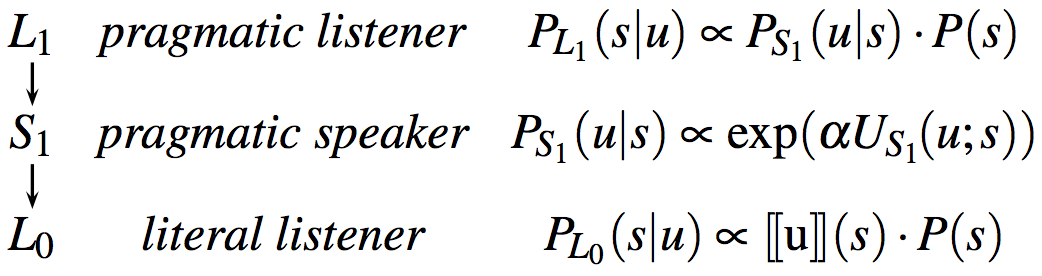
\includegraphics[width=0.5\linewidth]{vanilla-rsa.png}
	\end{center}
	\vspace{-0.3cm}
	\caption{A schematic depiction of a vanilla RSA model \parencite{problang}}
	\label{vanilla-rsa}
\end{figure*}
Putting all the elements together results in the vanilla version of an RSA-model (Fig. \ref{vanilla-rsa}).
 \pt{add actual numbers from the vanilla model}
%listener as updating beliefs -- example with L1 formula -- formal notion of S1 w example -- informativeness -- L0 
%note that these exist as part of L1's reasoning \parencite{lassiter2017adjectival}

“Speech acts are actions; thus, the speaker is modeled as a rational (Bayesian) actor. He chooses an action (e.g., an utterance) according to its utility. The speaker simulates taking an action, evaluates its utility, and chooses actions based on their utility. Rationality of choice is often defined as choice of an action that maximizes the agent’s (expected) utility. Here we consider a generalization in which speakers use a softmax function to approximate the (classical) rational choice to a variable degree” (problang)
The speaker chooses utterance u to communicate a state s to L0 , by trying to minimize effort for L0 to arrive from u at s, i.e., by minimizing surprisal of s given u, while trying to also keep utterance cost minimal. Having this utility function in mind, the S1 computes a probability distribution over utterances having an s in mind, in proportion to the speaker’s utility function Us (above), where alpha may control for speaker optimality  
“To interpret the utterance, the pragmatic listener considers the process that generated the utterance, in the first place” in the form of the S1. 


threshold semantics, where the threshold is probabilistically inferred \parencite{lassiter2017adjectival} for a given comparison class.

Lassiter \& Goodman (2013, 2017) first provided a model of gradable adjective interpretation within the RSA-framework, showing that a Bayesian approach can capture their vague meaning via inference over the latent threshold variable $\theta$ underlying the adjective semantics. Importantly, probabilistic reasoning provides tools to capture uncertainty over certain aspects of the message, in this particular case - the speaker’s intended meaning of the adjectival utterance.  
In the proposed model, the listener jointly infers the value of the threshold along with the state of the world - i.e., the degree of the propoerty under discussion. The literal meaning of adjectives is therefore formalised in terms of degree-semantics, assuming that the lexical entry of the adjective specifies the underlying scale and its polarity. 
The authors assume a standard RSA model with three levels, adding one crucial component - the threshold, entering the literal semantics of the adjective on the level of L0. 
In order to allow specifying the compositional semantics of the utterance via the L0 which requires the computation of the truth of an utterance for a given world state, the authors propose L1 consider all possible assignments of values the latent variable, given a prior over that variable. The assumed values are then iteratively passed down through the model, such that it can be computed how likely it is that S1 would produce the observed utterance if the threshold took on a particular value:
$$P_{L_0} (s | u, V) = P_{L_0} (s | \llbracket u \rrbracket ^V = 1 )$$

$$P_{S_1} (u | s, V) \propto exp(\alpha \times ln (P_{L_0} (s | u, V) - C(u)) )$$

Via Bayes' rule, L1 can then infer the joint posterior distribution over all possible combinations of states and values of the latent threshold:
$$P_{L_1} (s, V | u) \propto P_{S_1} (u | s, V) \times P_{L_1} (s) \times P_{L_1}(V)$$

In this work, the relevant comparison class was assumed to be implicitly supplied. 

QUD stuff

Tessler et al. 2017: 
Listeners use their world knowledge to infer the comparison class about what worlds are plausible given a specific comparison class, what comparison classes are likely to be talked about, and how a rational speaker would bhave in a given world and given a comparison class. 


\section{Refpred-RSA}
\pt{tbd}